\chapter{Selected Gamification Features for English Mind}

Through systematic analysis of existing language learning applications and their gamification implementations, this chapter presents a carefully curated selection of gamification features for English Mind. 

The selection methodology prioritized features that have demonstrated effectiveness in existing applications while maintaining strong alignment with English Mind's core pedagogical principles. Identified features strategically enhance two critical aspects of the learning experience:

\begin{enumerate}
    \item \textbf{Enhanced Practice Experience} 
    \begin{itemize}
        \item Diversified flashcard types
        \begin{itemize}
            \item Word spelling
            \item Word pronunciation
            \item Word-Definition matching
            \item Word-Translation matching
        \end{itemize}
        \item Post-practice review providing immediate feedback and reinforcement
        \item Individual word progress tracking breaking the abstract concept of SRS into tangible stages
    \end{itemize}
    
    \item \textbf{Consistent Practice Motivation} 
    \begin{itemize}
        \item A streak system requiring daily engagement with new vocabulary
    \end{itemize}
\end{enumerate}

\newpage
\section{Diversified Flashcard Types}

The current English Mind flashcard system uses a single format where users view an English word and recall its meaning. While effective, our analysis of similar applications revealed that incorporating multiple flashcard types can enhance engagement and address different aspects of vocabulary acquisition. We propose expanding the system to include five distinct flashcard types, each targeting specific learning objectives (see Figure \ref{fig:em-prototype-flashcard-types}).

\begin{itemize}
    \item \textbf{Basic Meaning Recognition (Existing)}

    The current format where users see an English word and recall its meaning will be maintained as the foundation of the practice system. This format effectively tests basic word recognition and meaning recall (see Section \ref{sec:em-active-recall-flashcards}).

    \item \textbf{Word Matching (Two Variants)}
    
    Following the successful implementation in applications like Duolingo and WordUp, we propose two matching exercise variants:
    
    \begin{itemize}
        \item \textbf{Word-Translation Matching:} Users match English words with their corresponding translations, presented in sets of five pairs.
        
        \item \textbf{Word-Definition Matching:} Similar to the translation variant, but users match English words with their definitions, reinforcing deeper understanding of word meanings.
    \end{itemize}

    \item \textbf{Word Spelling}
    
    This exercise type presents users with a word's definition and a contextual sentence containing a blank space. Users must correctly spell the target word to complete the sentence. To assist learning, an audio pronunciation button is available. The system evaluates spelling accuracy and provides immediate feedback.
    \newpage

    \item \textbf{Word Pronunciation}

    Users are shown an English word and prompted to pronounce it correctly. The flashcard displays both the word and its IPA (International Phonetic Alphabet) transcription. The system evaluates pronunciation accuracy using speech recognition technology, providing binary feedback (correct/incorrect). Understanding that not all practice environments are suitable for speaking exercises, users can opt to skip these cards when needed.

\end{itemize}

\begin{figure}[!h]
    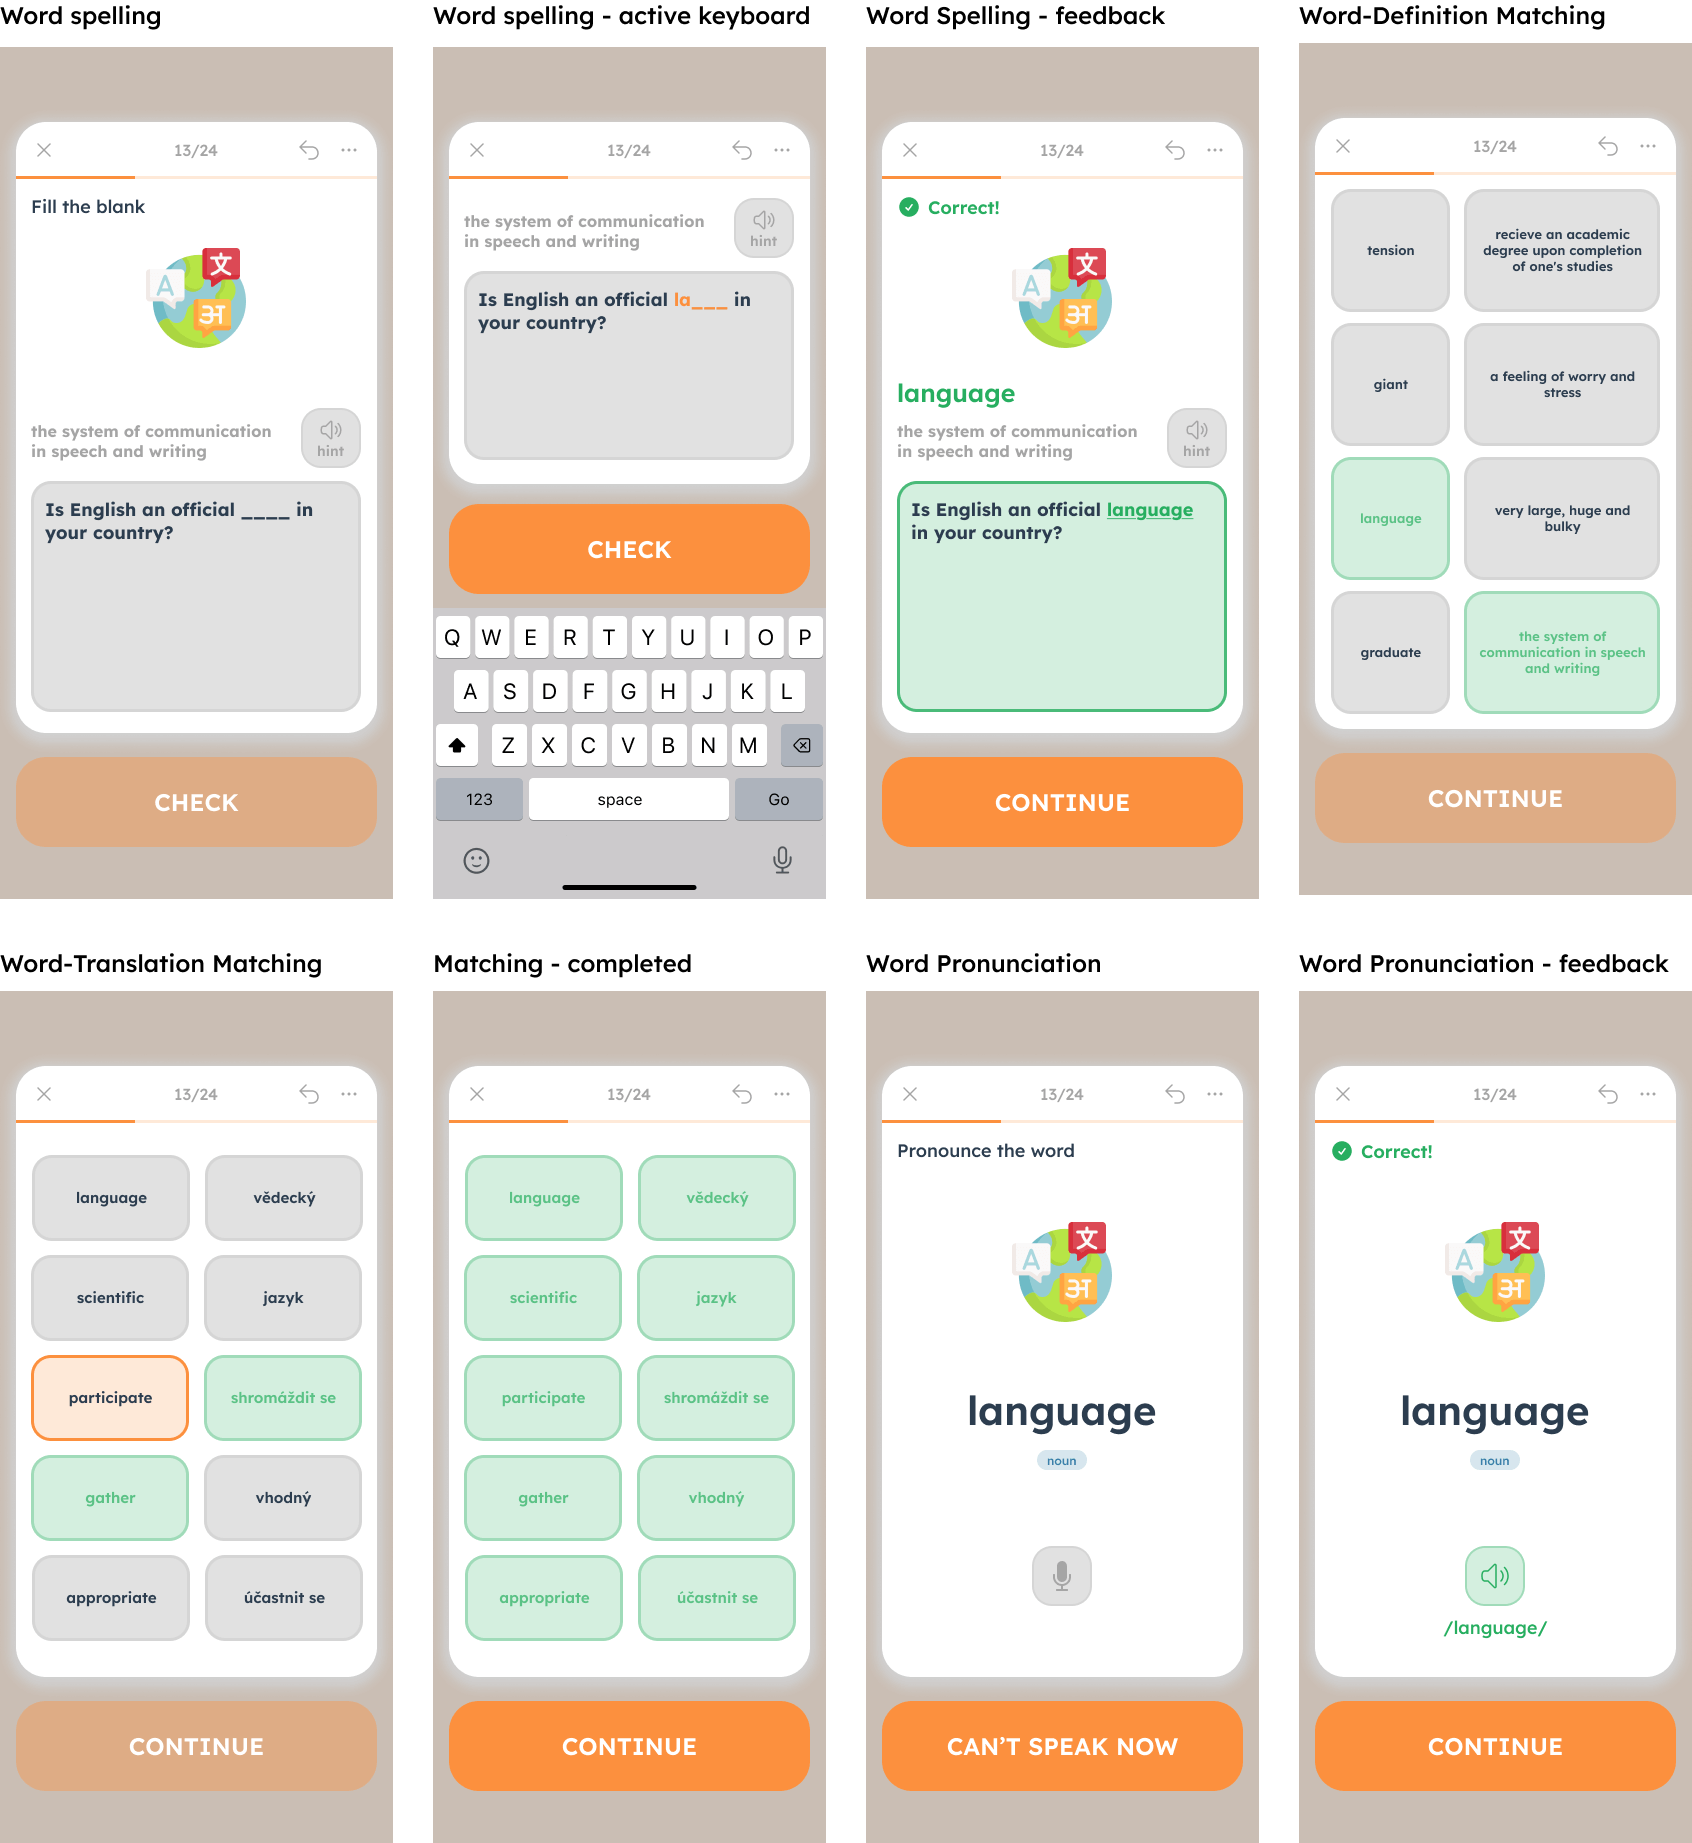
\includegraphics[width=1\textwidth]{src/figures/em-prototype-flashcards.png}
    \caption{English Mind - Prototype: Flashcard Types}
    \label{fig:em-prototype-flashcard-types}
\end{figure}

\subsection*{Implementation Considerations}

The integration of new flashcard types requires careful consideration of both the spaced repetition system and the distribution of different card types during practice sessions.

To maintain the integrity of the existing spaced repetition system, only the basic meaning recognition flashcards will carry spaced repetition metadata and influence the scheduling of words. The additional flashcard types will serve as supplementary practice exercises without affecting the core SRS algorithm. This approach ensures the proven effectiveness of the current SRS remains unchanged, while additional practice types enhance learning without disrupting the established review schedule. Furthermore, this design allows user progress tracking to remain clear and consistent throughout the learning process.

The distribution of flashcard types within a practice session follows a structured approach that ensures varied practice while maintaining focus on core vocabulary acquisition through the primary flashcard type:

\begin{itemize}
    \item \textbf{Primary Flashcards:} Basic meaning recognition flashcards appear first in the daily queue, maintaining their role as the foundation of the spaced repetition learning system.
    
    \item \textbf{Supplementary Flashcards:} After completing the primary flashcards, users encounter the following types in randomized order:
    \begin{itemize}
        \item \textbf{Matching Flashcards:} Appear once for every five words in practice, grouping words into logical sets
        \item \textbf{Spelling Flashcards:} Randomly distributed throughout the supplementary practice
        \item \textbf{Pronunciation Flashcards:} Limited to newly introduced words and appear less frequently than other types
    \end{itemize}
\end{itemize}

\subsection*{Expected Impact}

The diversification of flashcard types is expected to yield several benefits:

\begin{itemize}
    \item \textbf{Enhanced Engagement:} Variety in flashcard types reduces monotony and maintains user interest throughout longer practice sessions.
    
    \item \textbf{Comprehensive Learning and Retention:} Encountering words through diverse flashcard types (recognition, matching, spelling, and pronunciation) creates multiple memory pathways, leading to stronger and longer-lasting vocabulary mastery.
    
\end{itemize}

\section{Word Progress Tracking}

Building upon the success of WordUp's individual word progress tracking (see Section \ref{sec:wordup-individual-word-progress-experience}), we propose implementing a visual progress indicator system that integrates seamlessly with English Mind's existing spaced repetition system. This feature provides users with clear, immediate feedback on their progress with each vocabulary item, helping them understand where they stand in the learning journey for specific words.

\subsection*{Five-Stage Progress System}

The visual indicator system maps the existing spaced repetition intervals into five distinct stages. This system serves purely as a user-friendly representation of progress and does not modify the underlying SRS algorithm:


\begin{itemize}
    \item \textbf{Starting (Stage 1)}
    
    Represents words in their first 24 hours after introduction. These words are in the early stages of learning and require frequent review to establish basic recognition.
    
    \item \textbf{Familiarizing (Stage 2)}
    
    Covers words practiced between 1 day and 1 week. During this stage, words still require frequent reviews to build early recall strength and establish memory patterns.
    
    \item \textbf{Reinforcing (Stage 3)}
    
    Includes words with review intervals of 1-3 weeks. At this stage, users can recall words reliably, demonstrating consistent retention with moderate repetition intervals.
    
    \item \textbf{Strengthening (Stage 4)}
    
    Represents words practiced at 3-week to 3-month intervals. Users show strong confidence in recall, requiring significantly less frequent review as the word becomes well-established in long-term memory.
    
    \item \textbf{Almost Mastered (Stage 5)}
    
    Indicates words that have reached intervals of 3-8 months between reviews. These words are approaching full mastery, requiring only rare reviews to maintain retention. Once a word exceeds the 8-month interval, it will be marked as "known" and graduate from the regular review system.
\end{itemize}

\subsection*{Visual Implementation}

The progress indicator appears in the top-left corner of primary flashcards (see Figure \ref{fig:em-prototype-word-progress}). It consists of five sequential boxes that fill progressively as the word advances through the stages, providing an intuitive visualization of progress. This design choice ensures the indicator is visible but not distracting from the primary learning task.

\begin{figure}[!h]
    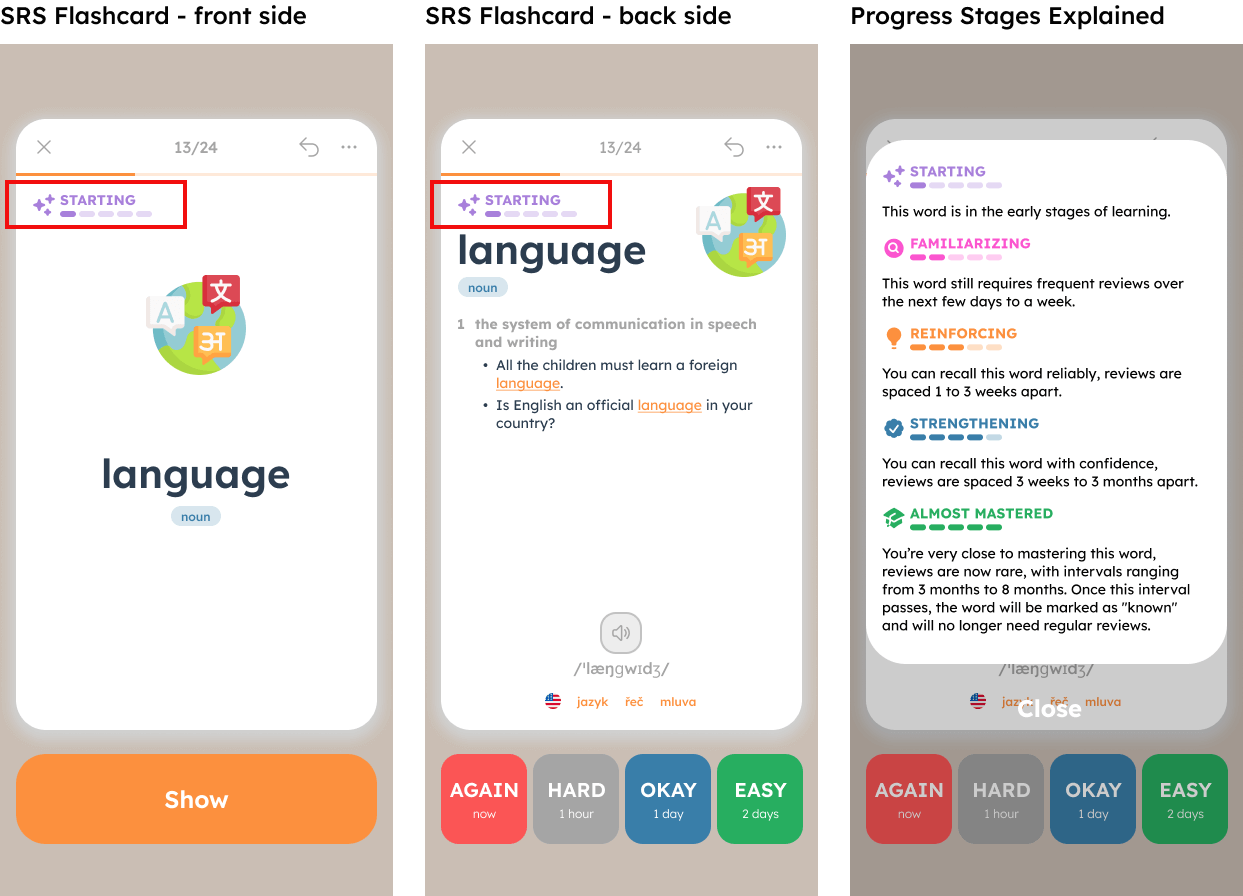
\includegraphics[width=1\textwidth]{src/figures/em-prototype-progress-system.png}
    \caption{English Mind - Prototype: Individual Word Progress Indicator (highlighted in red)}
    \label{fig:em-prototype-word-progress}
\end{figure}

\subsection*{Integration with Existing SRS}

The progress tracking system is designed to work in harmony with the existing spaced repetition algorithm. Progress stages are determined automatically based on the word's current interval in the SRS system, with stages advancing or regressing according to review performance. This implementation leverages existing SRS metadata, requiring minimal additional computational overhead.

\subsection*{Expected Impact}

The implementation of individual word progress tracking is expected to provide several benefits:

\begin{itemize}
    \item \textbf{Enhanced Motivation and Engagement:} Visual progress indicators create a game-like element that provides a sense of achievement as words advance through different stages.
    
    \item \textbf{Simplified Learning Metrics:} The staged system provides tangible feedback on the learning journey, making abstract concepts like spaced repetition more concrete and understandable.
\end{itemize}

\section{Post-Practice Review}

Drawing inspiration from Duolingo's successful implementation of post-practice feedback (see Section \ref{sec:duolingo-lesson-review}), we propose adding an engaging post-practice summary screen to English Mind. This feature provides immediate feedback and reinforcement after completing a practice session, helping users track their progress and maintain motivation.

\subsection*{Post-Practice Review Screen Components}

The post-practice review screen consists of several key elements (see Figure \ref{fig:em-prototype-practice-review}):

\begin{itemize}
    \item \textbf{Practice Statistics}
    
    Clear visualization of practice session metrics including the number of words practiced and time spent practicing.
    
    \item \textbf{Mascot Interaction}
    
    The app's mascot appears with randomly selected poses to add personality to the user experience.
    
    \item \textbf{Motivational Messages}
    
    A rotating collection of encouraging messages that vary based on factors such as the number of words practiced, time spent practicing, and time of day.
    
    \item \textbf{Celebratory Animation}
    
    A confetti animation plays when the review screen appears, providing immediate positive reinforcement for completing the practice session. The animation is optimized to ensure smooth and lightweight performance across different devices.
\end{itemize}

\begin{figure}[!h]
    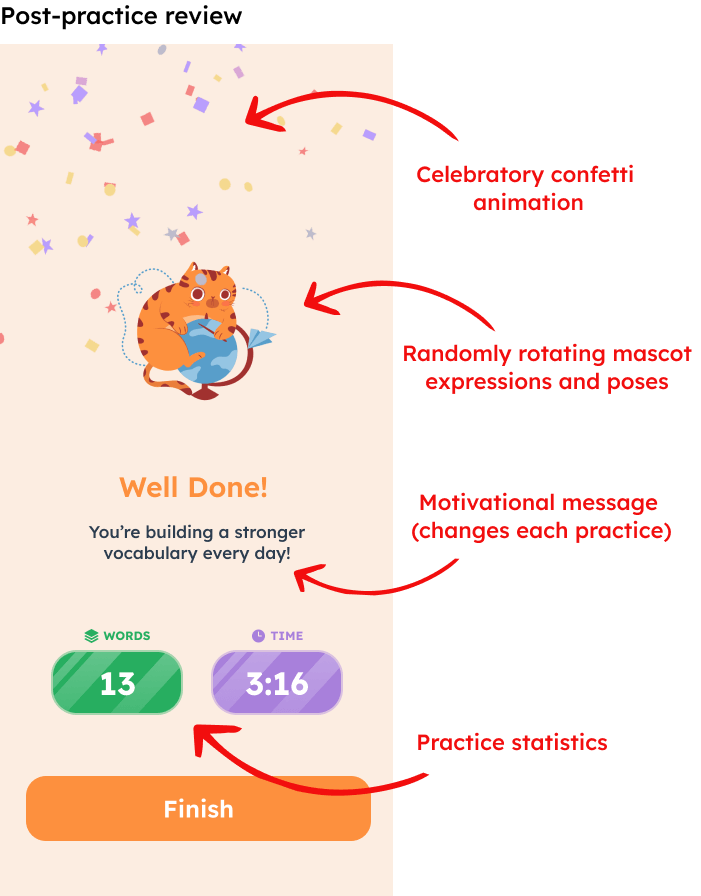
\includegraphics[width=0.8\textwidth]{src/figures/em-prototype-review.png}
    \caption{English Mind - Prototype: Post-Practice Review Screen}
    \label{fig:em-prototype-practice-review}
\end{figure}

\subsection*{Expected Impact}

The implementation of a post-practice review screen is expected to:

\begin{itemize}
    \item \textbf{Increase Practice Completion:} The anticipation of positive feedback and celebration may motivate users to complete their practice sessions.
    
    \item \textbf{Boost User Satisfaction:} Immediate positive reinforcement through animations and encouraging messages creates a more rewarding experience.
\end{itemize}

\section{Streak System}

The streak system is built on the fundamental requirement of learning at least one new word each day to maintain an active streak. Users must mark at least one word as "learning" each day and then review it at their daily queue of flashcards.This requirement ensures meaningful progress while keeping the daily commitment manageable for users. 

To support the effectiveness of the spaced repetition system, new words are strategically placed at the end of the review queue. This placement naturally encourages users to complete their due reviews before accessing the newly added words.

The system intentionally adopts a simplified approach, omitting streak features like "freeze" or streak recovery options. This deliberate choice allows us to establish and validate the core streak mechanics first, while features like streak freezes could be introduced in future iterations based on user feedback and engagement patterns.

\subsection*{Visual Implementation}

The streak counter is prominently displayed at the top of the main screen (see Figure \ref{fig:em-prototype-streak}). This implementation includes a clear numerical display of consecutive practice days, with visual states that reflect the streak's status: a bright, golden appearance for active streaks, and a faded, shadowed appearance when the streak is at risk of being lost.

Upon completing the daily flashcard practice and increasing the streak, a celebration screen appears to reinforce the user's achievement (see Figure \ref{fig:em-prototype-streak}). This screen showcases the updated streak count alongside a weekly progress view displaying the current week's streak activity (Monday through Sunday). When users maintain a perfect week of daily practice, these seven days are highlighted within a special golden frame, providing additional visual recognition for consistent engagement.

\newpage

\begin{figure}[!h]
    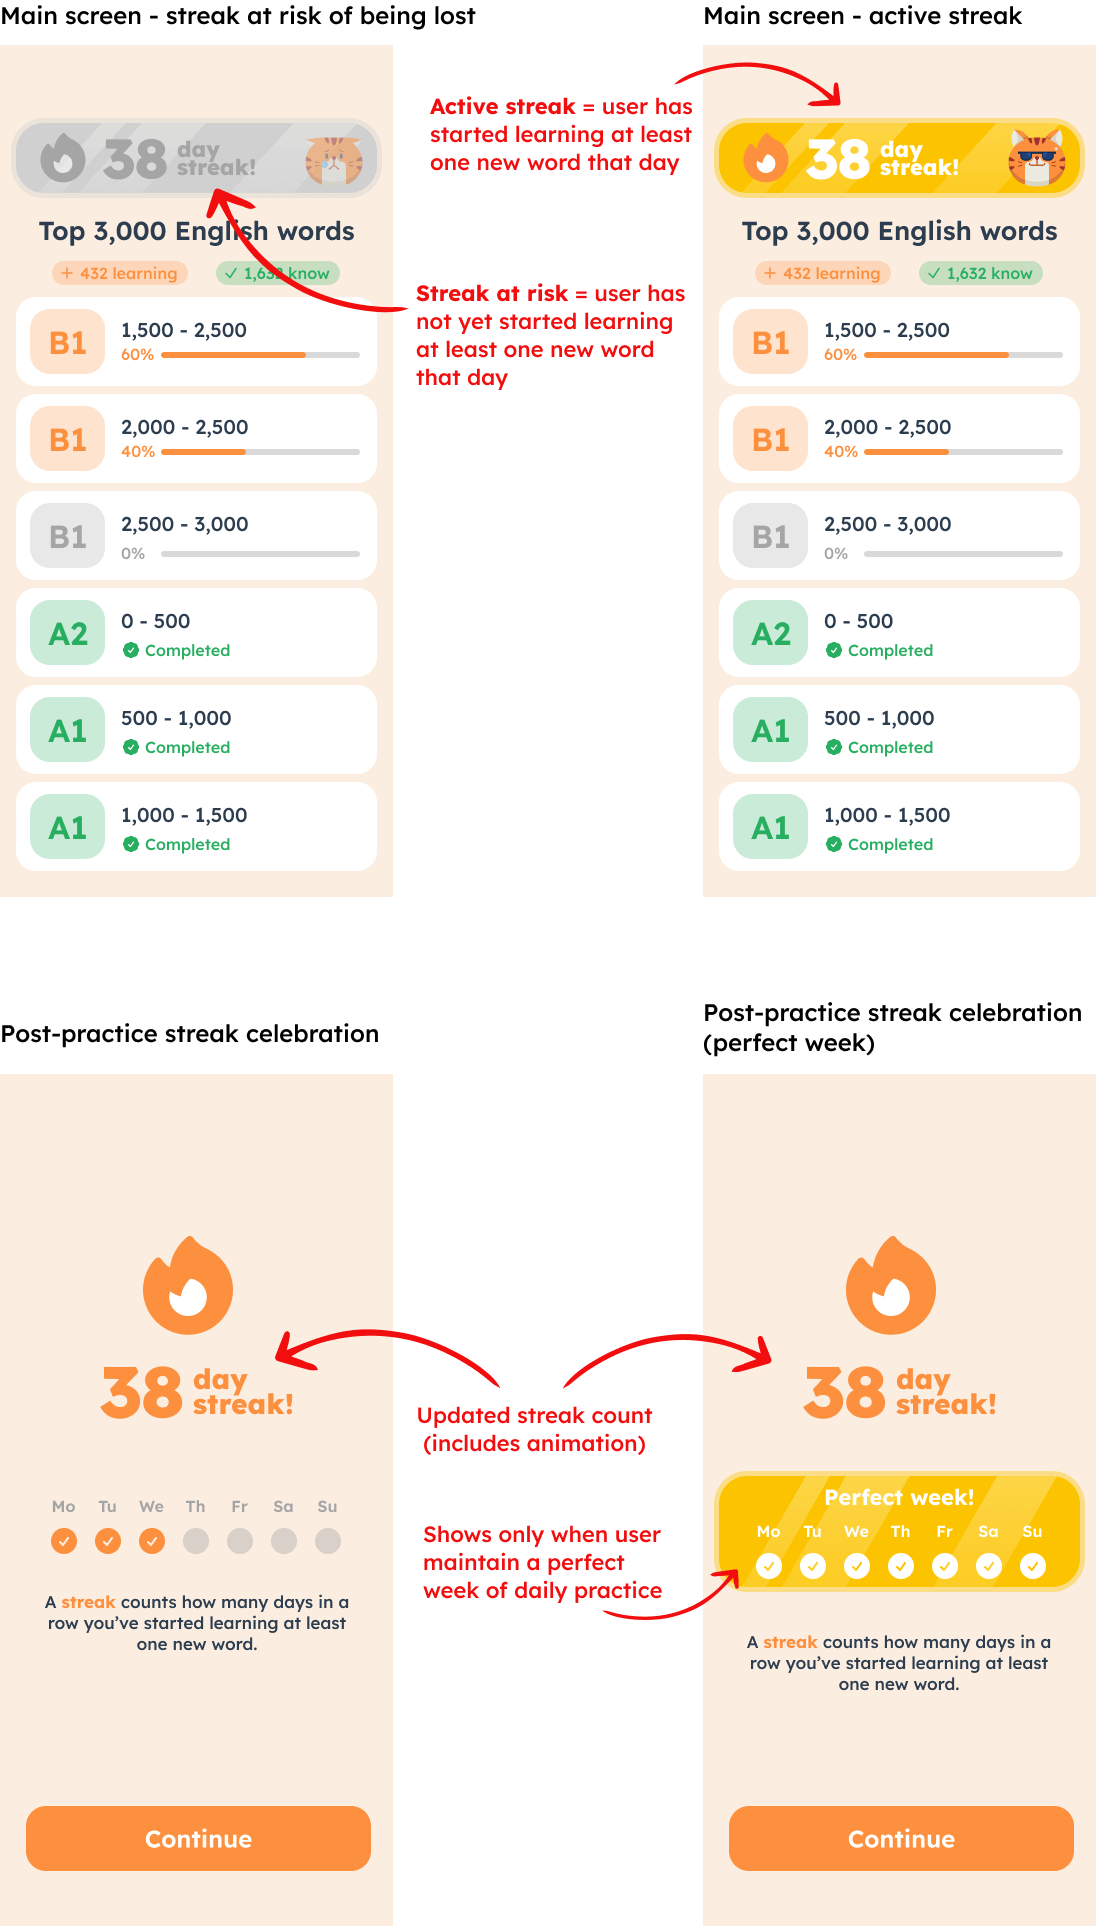
\includegraphics[width=0.9\textwidth]{src/figures/em-prototype-streak.png}
    \caption{English Mind - Prototype: Streak Implementation}
    \label{fig:em-prototype-streak}
\end{figure}

\subsection*{Expected Impact}

The streak system is designed to serve multiple pedagogical and motivational purposes:

\begin{itemize}
    \item \textbf{Establish Daily Practice Habits:} By providing a clear, visible metric for consistency, it helps users establish and maintain daily practice habits.
    
    \item \textbf{Encourage Complete Reviews:} The strategic placement of new words after due flashcards naturally encourages users to complete their spaced repetition queue.
\end{itemize}
